\documentclass[11pt,a4paper]{article}
\usepackage[utf8]{inputenc}
\usepackage[T1]{fontenc}
\IfFileExists{lmodern.sty}{\usepackage{lmodern}}{}
\IfFileExists{french.ldf}{\usepackage[french]{babel}}{\usepackage[english]{babel}}
\usepackage{amsmath,amssymb,amsfonts,amsthm}
\usepackage{geometry}
\geometry{top=2cm, bottom=2cm, left=2.2cm, right=2.2cm}
\usepackage{booktabs,array,multirow}
\usepackage{enumitem}
\usepackage{xcolor}
\usepackage{tcolorbox}
\tcbuselibrary{skins,breakable}
\usepackage{tikz}
\usetikzlibrary{arrows.meta,positioning,shapes.geometric,calc}
\usepackage[colorlinks=true,linkcolor=blue!60!black]{hyperref}
\newtcolorbox{propbox}[1]{colback=blue!5!white,colframe=blue!75!black,fonttitle=\bfseries,title={#1},breakable,boxrule=0.8pt}
\newtcolorbox{rembox}[1]{colback=orange!5!white,colframe=orange!80!black,fonttitle=\bfseries,title={#1},breakable,boxrule=0.8pt}
\newtcolorbox{verifbox}{colback=green!4!white,colframe=green!45!black,fonttitle=\bfseries,title=Vérification algorithmique (Python),breakable,boxrule=0.6pt}
\newcommand{\Xt}{\tilde{X}}
\newcommand{\Yt}{\tilde{Y}}
\setlength{\parindent}{0pt}
\setlength{\parskip}{4pt}
\title{\textbf{Université Akli Mohand Oulhadj -- Bouira}\\
\large Master Recherche Opérationnelle (RO) -- 2025/2026\\
\Large \textbf{Théorie des Jeux : Corrigé détaillé du Contrôle Continu (3h)}}
\author{\textbf{Référence de cours :} Chapitre 1 (jeux matriciels)\\ Chapitre 2 (jeux antagonistes infinis, équilibre de Nash)}
\date{}

\begin{document}
\maketitle
\hrule
\vspace{0.3cm}
\textbf{Barème indicatif} (aligné sur le corrigé officiel du DM1) : Ex.~1, jeu $J$ (7 pts) ; jeu $J'$ (8 pts) ; Ex.~2 (5 pts).

%=====================================================================
\section*{Exercice 1 -- Jeu $J$}
\[
A=\begin{pmatrix}1&3&0\\2&1&4\end{pmatrix}\qquad\text{(gains du joueur 1, qui maximise ; le joueur 2 minimise).}
\]

\subsection*{1. Solution en stratégies pures ? \hfill[1 pt]}
\begin{align*}
\min_j a_{1j}&=\min\{1,3,0\}=0,\quad \min_j a_{2j}=\min\{2,1,4\}=1\ \Rightarrow\ \alpha=\max_i\min_j a_{ij}=1,\\
\max_i a_{i1}&=2,\quad\max_i a_{i2}=3,\quad\max_i a_{i3}=4\ \Rightarrow\ \beta=\min_j\max_i a_{ij}=2.
\end{align*}
$\alpha=1<2=\beta$ : aucun élément n'est à la fois minimal dans sa ligne et maximal dans sa colonne.
\[\boxed{J \text{ n'admet pas de solution en stratégies pures.}}\]

\subsection*{2. Extension mixte \hfill[1 pt]}
\[
\Xt=\{x\in\mathbb{R}^2_+ : x_1+x_2=1\},\quad \Yt=\{y\in\mathbb{R}^3_+ : y_1+y_2+y_3=1\},
\]
\[
E(x,y)=x^TAy=\sum_{i,j}a_{ij}x_iy_j=x_1y_1+3x_1y_2+2x_2y_1+x_2y_2+4x_2y_3,
\]
$\tilde J=\langle I=\{1,2\},\Xt,\Yt,E\rangle$ : J1 maximise $E$, J2 minimise $E$.

\subsection*{3. Stratégie optimale du joueur 1 \hfill[2,5 pts]}
\paragraph{Méthode graphique.} $x=(p,1-p)$. Gains contre chaque colonne :
\[
C_1:\ p+2(1-p)=2-p,\qquad C_2:\ 3p+(1-p)=1+2p,\qquad C_3:\ 4(1-p)=4-4p.
\]
J1 maximise $\varphi(p)=\min\{2-p,\,1+2p,\,4-4p\}$ sur $[0,1]$.
\begin{center}
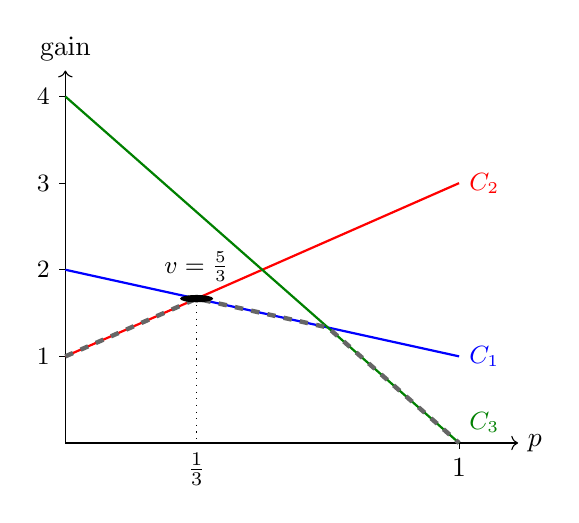
\begin{tikzpicture}[xscale=5,yscale=1.1]
\draw[->] (0,0)--(1.15,0) node[right]{$p$};
\draw[->] (0,0)--(0,4.3) node[above]{gain};
\foreach \y in {1,2,3,4} \draw (0,\y)--(-0.015,\y) node[left]{\small\y};
\draw (1,0)--(1,-0.07) node[below]{$1$};
\draw[blue,thick] (0,2)--(1,1) node[right]{\small $C_1$};
\draw[red,thick] (0,1)--(1,3) node[right]{\small $C_2$};
\draw[green!50!black,thick] (0,4)--(1,0) node[above right]{\small $C_3$};
\draw[ultra thick,black!60,dashed] (0,1)--(1/3,5/3)--(2/3,4/3)--(1,0);
\fill (1/3,5/3) circle (1.2pt);
\draw[dotted] (1/3,5/3)--(1/3,0) node[below]{$\frac13$};
\node[above] at (1/3,1.75) {\small $v=\frac53$};
\end{tikzpicture}
\end{center}
L'enveloppe inférieure vaut $1+2p$ sur $[0,\frac13]$, $2-p$ sur $[\frac13,\frac23]$, $4-4p$ sur $[\frac23,1]$. Son maximum est en $2-p=1+2p\iff p=\frac13$, valeur $\frac53$ ; et $C_3$ y vaut $4-\frac43=\frac83>\frac53$.

\paragraph{Contrôle par la programmation linéaire (cours p.~27--28).} $v\ge\alpha=1>0$ ; avec $P_i=x_i/v$ :
\[
(I')\ \begin{cases}P_1+P_2\to\min\\ P_1+2P_2\ge1\ (\Delta_1),\quad 3P_1+P_2\ge1\ (\Delta_2),\quad 4P_2\ge1\ (\Delta_3)\\ P_1,P_2\ge0\end{cases}
\]
Optimum en $\Delta_1\cap\Delta_2$ : $(P_1,P_2)=(\frac15,\frac25)$, et $4P_2=\frac85>1$. Donc $v=\frac{1}{P_1+P_2}=\frac53$, $x=(P_1v,P_2v)=(\frac13,\frac23)$.
\[
\boxed{x^*=\Big(\frac13,\frac23\Big),\qquad v=\frac53\ :\ \text{J1 s'assure un gain moyen d'au moins } \tfrac53.}
\]

\subsection*{4. Stratégie optimale du joueur 2 \hfill[2,5 pts]}
Contre $x^*$, $C_3$ donne $\frac83>v$ : par les écarts complémentaires ($4P_2>1\Rightarrow q_3=0$), $y_3^*=0$. Avec $y=(q,1-q,0)$ :
\[
L_1:\ q+3(1-q)=3-2q,\qquad L_2:\ 2q+(1-q)=1+q;\qquad 3-2q=1+q\iff q=\tfrac23.
\]
(Dual : $q_1+3q_2=1$, $2q_1+q_2=1\Rightarrow q=(\frac25,\frac15,0)$, $y=qv$.)
\[
\boxed{y^*=\Big(\frac23,\frac13,0\Big),\qquad \text{perte maximale } \tfrac53,\ \text{gain optimal de J2 } =-\tfrac53.}
\]
\textbf{Vérification (Théorème 2).} $E(L_1,y^*)=\frac23+1=\frac53$, $E(L_2,y^*)=\frac43+\frac13=\frac53$ ; $x^{*T}A=(\frac53,\frac53,\frac83)\ge\frac53$. \checkmark

%=====================================================================
\section*{Exercice 1 (suite) -- Jeu $J'$}
\[
A'=\begin{pmatrix}2&6&5&0\\4&2&3&8\\4&2&2&6\\2&4&4&2\end{pmatrix}.
\]

\subsection*{1. La stratégie 3 du joueur 1 est-elle dominée ? \hfill[1 pt]}
$L_2=(4,2,3,8)$ et $L_3=(4,2,2,6)$ : $L_2\ge L_3$ composante par composante, avec $3>2$ et $8>6$.
\[\boxed{L_3 \text{ est dominée (au sens large) par } L_2.}\]
La domination n'est \emph{pas stricte} (égalités en colonnes 1 et 2).

\subsection*{2. $L_4$ strictement dominée dans l'extension mixte \hfill[2 pts]}
Cherchons $\lambda\in[0,1]$ avec $\lambda L_1+(1-\lambda)L_2>L_4=(2,4,4,2)$ :
\[
\begin{array}{lll}
C_1: & 2\lambda+4(1-\lambda)=4-2\lambda>2 & \iff\lambda<1\\
C_2: & 6\lambda+2(1-\lambda)=2+4\lambda>4 & \iff\lambda>\frac12\\
C_3: & 5\lambda+3(1-\lambda)=3+2\lambda>4 & \iff\lambda>\frac12\\
C_4: & 8(1-\lambda)=8-8\lambda>2 & \iff\lambda<\frac34
\end{array}
\]
Tout $\lambda\in\,]\frac12,\frac34[$ convient. Pour $\lambda=\frac23$ :
\[
\tfrac23L_1+\tfrac13L_2=\Big(\tfrac83,\tfrac{14}3,\tfrac{13}3,\tfrac83\Big)>(2,4,4,2)=L_4.
\]
\[\boxed{L_4 \text{ est strictement dominée par la stratégie mixte } (\tfrac23,\tfrac13,0,0).}\]

\emph{Remarque :} aucune stratégie pure ne domine $L_4$ ($L_1$ a $0<2$ en $C_4$ ; $L_2$ a $2<4$ en $C_2$ ; $L_3$ a $2<4$ en $C_2$). L'extension mixte est indispensable.

\subsection*{3. Après suppression de $L_3,L_4$ : $C_3$ strictement dominée \hfill[2 pts]}
\[
A''=\begin{pmatrix}2&6&5&0\\4&2&3&8\end{pmatrix}.
\]
J2 minimise : on cherche $\mu\in[0,1]$ avec $\mu C_1+(1-\mu)C_2<C_3=(5,3)^T$ :
\[
L_1:\ 2\mu+6(1-\mu)=6-4\mu<5\iff\mu>\tfrac14,\qquad L_2:\ 4\mu+2(1-\mu)=2+2\mu<3\iff\mu<\tfrac12.
\]
Pour $\mu=\frac13$ : $\frac13C_1+\frac23C_2=(\frac{14}3,\frac83)^T<(5,3)^T$.
\[\boxed{C_3 \text{ est strictement dominée par la stratégie mixte } (\tfrac13,\tfrac23,0,0) \text{ du joueur 2.}}\]

\subsection*{4. Solution du jeu réduit, puis de $J'$ \hfill[3 pts]}
Jeu réduit (lignes $L_1,L_2$ ; colonnes $C_1,C_2,C_4$) :
\[
\begin{pmatrix}2&6&0\\4&2&8\end{pmatrix}=2A.
\]
\textbf{Joueur 1}, $x=(p,1-p)$ : $C_1:4-2p$, $C_2:2+4p$, $C_4:8-8p$. Maximum de l'enveloppe inférieure en $2+4p=4-2p\iff p=\frac13$, $v=\frac{10}{3}$ ; $C_4$ y vaut $\frac{16}3>\frac{10}3$.

\textbf{Joueur 2} : $C_4$ non jouée ; $(q,1-q,0)$ : $L_1:6-4q$, $L_2:2+2q$, égalité pour $q=\frac23$, $v=\frac{10}3$.

(Contrôle : par l'invariance affine du DM1 Ex.~2, $2A$ a les mêmes stratégies optimales que $A$ et la valeur $2\cdot\frac53=\frac{10}3$.)

\textbf{Retour à $J'$} : on remet des zéros sur les stratégies éliminées (proposition p.~19 du cours) :
\[
\boxed{x^*=\Big(\frac13,\frac23,0,0\Big),\qquad y^*=\Big(\frac23,\frac13,0,0\Big),\qquad v(J')=\frac{10}3.}
\]
\textbf{Vérification dans $J'$ (Théorème 2).}
$x^{*T}A'=\big(\frac{10}3,\frac{10}3,\frac{11}3,\frac{16}3\big)\ge\frac{10}3$ ;
$A'y^*=\big(\frac{10}3,\frac{10}3,\frac{10}3,\frac83\big)^T\le\frac{10}3$. Le couple $(x^*,y^*)$ est un point selle de l'extension mixte de $J'$. \checkmark

\begin{rembox}{Remarque}
L'élimination d'une stratégie seulement faiblement dominée ($L_3$) conserve la valeur et fournit une solution optimale, mais ne garantit pas d'obtenir toutes les solutions optimales (ici $L_3$ rapporte aussi $\frac{10}3$ contre $y^*$).
\end{rembox}

%=====================================================================
\section*{Exercice 2 -- Jeu continu \hfill[5 pts]}
$X_1=X_2=[-1,1]$, $f_1(x_1,x_2)=-x_1^2+2x_1x_2$, $f_2(x_1,x_2)=-x_2^2+2x_1x_2$.

\subsection*{1. Conditions du théorème de Nash \hfill[1,5 pt]}
\begin{itemize}
\item $X_i=[-1,1]$ est non vide, compact (fermé borné) et convexe. \checkmark
\item $f_1$, $f_2$ polynomiales, donc continues sur $X_1\times X_2$. \checkmark
\item $\frac{\partial^2f_1}{\partial x_1^2}=-2<0$ : $x_1\mapsto f_1(x_1,x_2)$ concave pour tout $x_2$ ; de même $\frac{\partial^2f_2}{\partial x_2^2}=-2<0$. \checkmark
\end{itemize}
\[\boxed{\text{Les conditions sont vérifiées : le jeu admet au moins un équilibre de Nash.}}\]

\subsection*{2. Ensemble des issues \hfill[1 pt]}
$X=X_1\times X_2=[-1,1]^2$ : le carré plein de sommets $(\pm1,\pm1)$.
\begin{center}
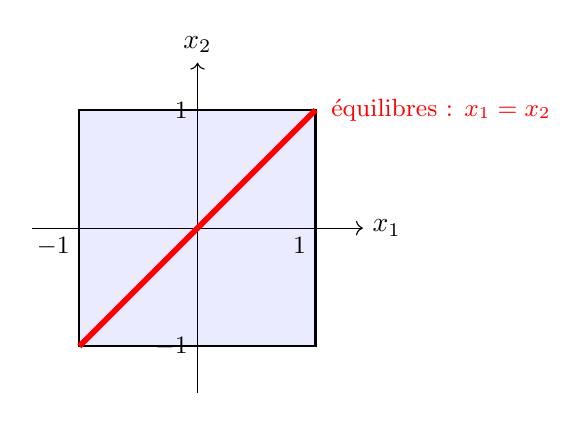
\begin{tikzpicture}[scale=1.5]
\fill[blue!8] (-1,-1) rectangle (1,1);
\draw[thick] (-1,-1) rectangle (1,1);
\draw[->] (-1.4,0)--(1.4,0) node[right]{$x_1$};
\draw[->] (0,-1.4)--(0,1.4) node[above]{$x_2$};
\node[below left] at (1,0) {\small $1$}; \node[below left] at (-1,0) {\small $-1$};
\node[left] at (0,1) {\small $1$}; \node[left] at (0,-1) {\small $-1$};
\draw[red,line width=2pt] (-1,-1)--(1,1);
\node[red,right] at (1.05,1) {\small équilibres : $x_1=x_2$};
\end{tikzpicture}
\end{center}

\subsection*{3. Équilibres de Nash \hfill[2,5 pts]}
\textbf{Meilleures réponses.} $\frac{\partial f_1}{\partial x_1}=-2x_1+2x_2=0\iff x_1=x_2$, qui appartient à $[-1,1]$ ; par stricte concavité c'est l'unique maximum : $R_1(x_2)=\{x_2\}$. Symétriquement $R_2(x_1)=\{x_1\}$.

\textbf{Intersection.} $x_1^*\in R_1(x_2^*)$ et $x_2^*\in R_2(x_1^*)\iff x_1^*=x_2^*$.
\[
\boxed{\mathcal{E}_{Nash}=\{(t,t):t\in[-1,1]\},\qquad f_1=f_2=t^2.}
\]
\textbf{Vérification.} $f_1(x_1,t)=t^2-(x_1-t)^2\le t^2=f_1(t,t)$, idem pour J2 : aucune déviation unilatérale n'est profitable. Les équilibres $(1,1)$ et $(-1,-1)$ (gains $(1,1)$) sont les seuls Pareto-optimaux parmi les équilibres.

\vspace{0.4cm}
\begin{verifbox}
Recontrôlé dans \texttt{verification\_TDJ.py} : $\alpha=1<\beta=2$ ; $(x^*,y^*,v)=((\frac13,\frac23),(\frac23,\frac13,0),\frac53)$ ; dominations $\frac23L_1+\frac13L_2>L_4$ et $\frac13C_1+\frac23C_2<C_3$ ; solution de $J'$ ($v=\frac{10}3$) en arithmétique exacte et par \texttt{linprog} ; meilleures réponses et diagonale d'équilibres de l'Ex.~2.
\end{verifbox}

\end{document}
